Since a point cloud is a 3D structure, it is quite natural using a 3D model as a projection space. In this section we will present an approach that projects the cloud points into a volumetric occupancy grids and, given these grids, performs the classification task using a 3D convolutional neural network: VoxNet.

\paragraph{Input}
The initial input of the algorithm is a point cloud segment, usually given by the intersection of a point cloud with a bounding box and may include background clutter. 

Each point $(x,y,z)$ of the point cloud is mapped to discrete voxel coordinates $(i,j,k)$. 
This mapping is obviously depending on the orientation, origin and resolution of the voxel grid in space. For the orientation it is assumed that the $z$ axis is aligned with the gravity direction, while the origin is supposed to be given as an input. How to deal with the remaining degree of freedom, the rotation around the $z$ axis? First method: it is possible to define a canonical orientation for each object and detect this orientation automatically, but this approach is often non-trivial in practise. Second method: using data augmentation at training time; in practise what we have to do is to create $n$ copies of each input instance, each rotated $360$\textdegree$/n$ around the $z$ axis. At testing time we pool the activations of the output layer over all $n$ copies. As mentioned, also grid resolution has influence on results: in the experiments a fixed occupancy grid $32 \times 32 \times 32$ voxels was used. We have to keep these dimensions small because the computational space increases cubically. To keep larger spatial extents in memory are used hierarchical data structures and copy specific segments to dense arrays as needed. 

There are three possible ways to model occupancy grids:
\begin{itemize}
\item \emph{Binary occupancy grid. } Each voxel has just two options, it can be occupied or unoccupied. Since data coming from sensors always is noisy a probabilistic approach is used to determine the voxel's binary state.
\item \emph{Density grid. } Identical to the previous one, except for the fact that each voxel is assumed to have a continuous, and not binary, density.
\item \emph{Hit grid. } Differently from the two previous approaches, this model only consider hits, and ignore the difference between unknown and free space. Hence the probabilistic approach is different.
\end{itemize}

\begin{figure}[ht]
    \centering
    \captionsetup{width=.9\linewidth}
    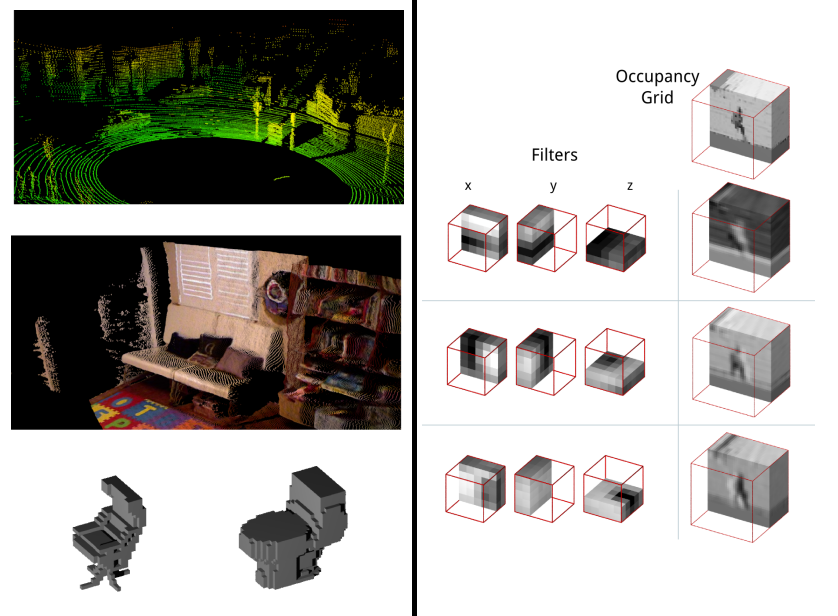
\includegraphics[width=0.72\textwidth]{images/VOLUM_cloud_filtpng.png}
    \caption{Left: From top to bottom, a point cloud from the Sydney Objects Dataset,
a point cloud from NYUv2, and two voxelized models from ModelNet40.
Right: Cross sections of three 5 × 5 × 5 filters from the first layer of VoxNet in the Sydney Objects Database, with corresponding feature map on the right.}
    \label{fig:VOLUM_cloud_filtpng}
\end{figure}

\paragraph{Architecture}
The input layer accepts a grid of $I \times J \times K$ voxels, as described before. In the performed experiments $I = J = K = 32$. Voxel entries are supposed to be normalized in the range $(-1,1)$.

After the input layer we have convolutional layers. The notation that will be used to describe these layers is $C(f,d,s)$, where $f$ is the number of filters, $d$ is the spatial dimension and $s$ is the stride. The output is passed through a leaky ReLU ($a(x)=max(0.1*x , x)
)$ with parameter 0.1.

Next we have pooling layers $P(m)$, used to downsample the input volume. We divided our input in blocks of $m \times m \times m$ and then take their maximum (we have a max-pooling operation).

At the end we have fully connected layers $FC(n)$, where $n$ is the number of output neurons. The activation function used are ReLUs and in the final layer it's used a softmax activation function.

An optimization of the hyperparameters leads to obtain the following network scheme:
$C(32, 5, 2) - C(32, 3, 1)-P(2)-F C(128)-F C(K)$, where $K$ is the number of classes (see figure \ref{fig:VoxNet_archtecture}). In total the model has $921736$ parameters, much less than a typical CNN for image classification. The authors of the paper think this is because point cloud classification is a simpler task, as many factors that images classifiers have to take into account (perspective, illumination, ...) are not present. Training details: SGD with momentum, L2 regularization, dropout, momentum parameter 0.9, initial LR=0.01 or 0.001 depending on the dataset.


It is also possible to use a multiresolution approach. In this case we use $r$ networks as described before, each of them corresponding to a resolution input grid. Then, at the fully connected layers, we merge informations coming from the different networks and obtain a single descriptor.

\begin{figure}[ht]
    \centering
    \captionsetup{width=.7\linewidth}
    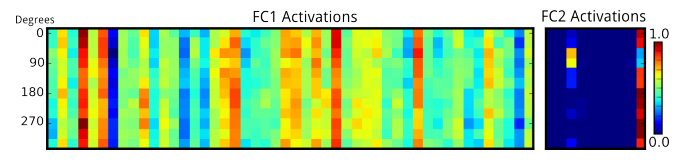
\includegraphics[width=0.6\textwidth]{images/VOLUM_invariance.png}
    \caption{Neuron activations for the two fully connected layers of VoxNet
when using the point cloud from figure \ref{fig:VoxNet_archtecture} (right) as input in 12 different
orientations.}
    \label{fig:VOLUM_invariance}
\end{figure}

\begin{figure}[ht]
    \centering
    \captionsetup{width=.9\linewidth}
    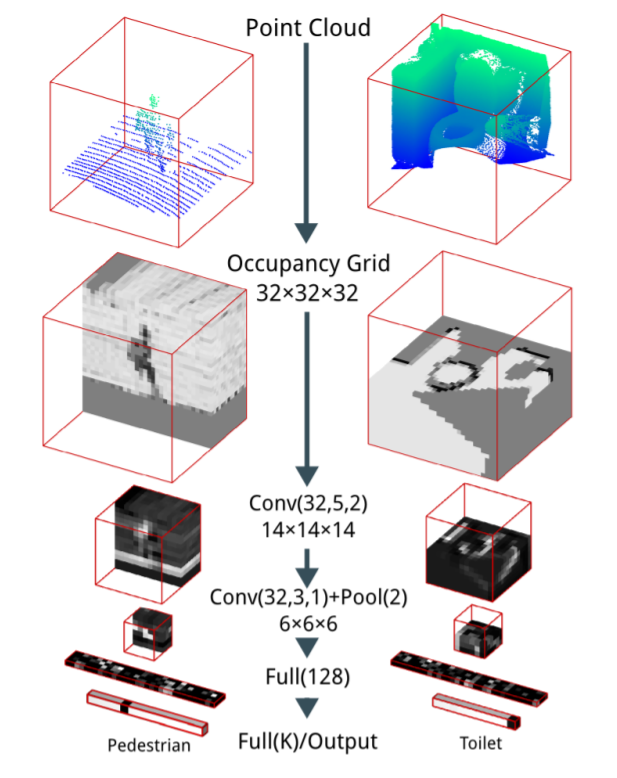
\includegraphics[width=0.4\textwidth]{images/VoxNet_archtecture.png}
    \caption{The VoxNet Architecture. We show inputs, example
feature maps, and predicted outputs for two instances from our experiments.
The point cloud on the left is from LiDAR and is part of the Sydney Urban
Objects dataset \cite{dataset_ICRA2012}. The point cloud on the right is from RGBD and is part of NYUv2 \cite{dataset_ECCV2012}.}
    \label{fig:VoxNet_archtecture}
\end{figure}

\paragraph{Results}
VoxNet was evalueted in three different domains: LiDAR point cloud, RGBD point clouds and CAD models as figure \ref{fig:VOLUM_cloud_filtpng} shows. In figure \ref{fig:VOLUM_results_table} are reported some results on different datasets and comparison to other approaches. 

\begin{figure}[ht]
    \centering
    \captionsetup{width=.9\linewidth}
    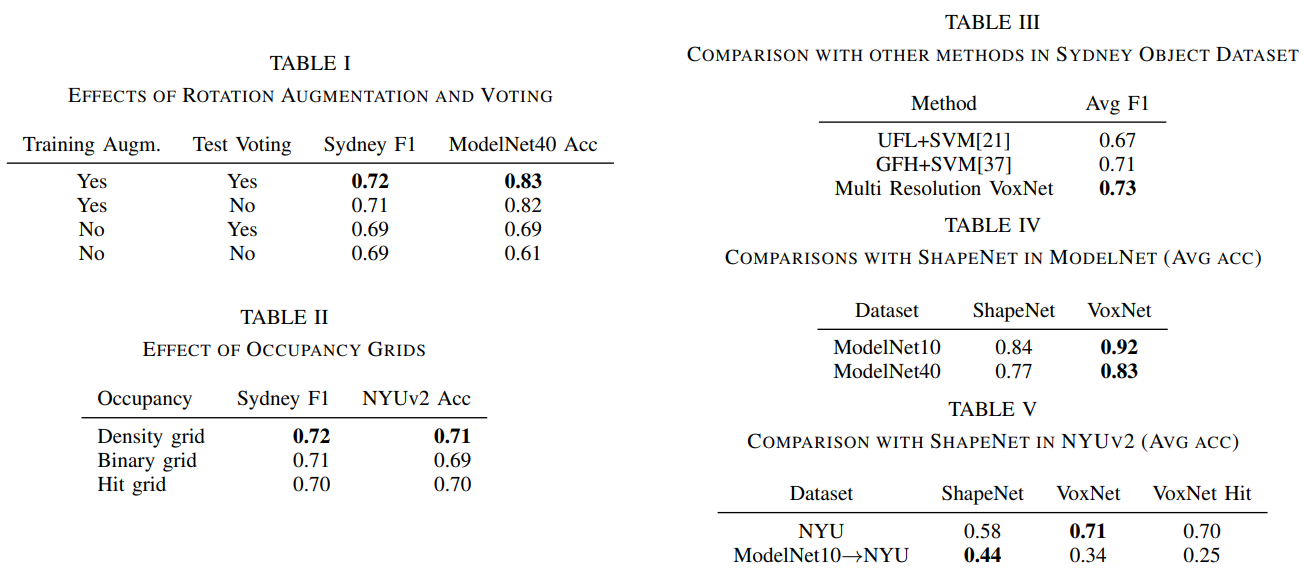
\includegraphics[width=0.9\textwidth]{images/VOLUM_results_table.png}
    \caption{Performance results on different datasets, and comparison to other approaches: UFL+SVM combines unsupervised Deep Learning with SVM; GFH+SVM designs a rotationally invariant descriptor and classifies it with a nonlinear SVM.}
    \label{fig:VOLUM_results_table}
\end{figure}

A qualitative result we can test is the rotational invariance. As explained before, the network was trained using data augmentation (pre-established rotation around $z$ axis). In order to verify if there is an effective rotational invariance we can analyze the activation of the two fully connected layers, given as input the same point cloud in different orientations. As we can see in figure \ref{fig:VOLUM_invariance}, 12 different rotation are analyzed and the corresponding neuron activation are very similar. This show that there is an approximate rotational invariance.